\chapter{局部凸函数三角化} \label{chap:LCT}
本章首先在\ref{sec:ODT}节中回顾了最优Delaunay三角化,然后在\ref{sec:LCT}节中介绍局部凸函数三角化算法,最后在\ref{sec:other_criteria}节中介绍如何联合一些其他的准则对目标各向异性网格进行边长的控制和几何误差控制。

\section{最优Delaunay三角化回顾} \label{sec:ODT}
Chen等在\cite{Chen2004,Chen2007}中提出了最优Delaunay三角化算法(ODT),他们将各向异性网格生成问题转化为一个函数逼近的问题。设一个网格(三角形网格与四面体网格)为$\mT = \bigcup_{k=1}^N \tau_k$,其中$\tau_k$是网格$\mT$中的第$k$ 个单元(单元指三角形或者四面体)。在定义域$\Omega \in \mR^d, \, d\geq 2$上给定一个函数$u: \mR^d \rightarrow \mR $,ODT在给定顶点数的前提下,去寻找一个定义在$\Omega$上的网格$\mT$,使得$u$和$\hat{u}$ 之间$L^p$ 误差最小。$\hat{u}$ 是$u$在$\mT$上的分段线性逼近函数。更进一步,ODT的误差定义为
\begin{equation} \label{eqn:odtformula}
E_{ODT,u,p} \triangleq \| \hat{u} - u\|_{L^p} = \left(\sum_{\tau \in \mT}\int_{\tau} |\hat{u}(\mx) - u(\mx)|^p\, \mathrm{d} \mx\right)^{1/p}.
\end{equation}
当$u$是一个凸函数时,$E_{ODT,u,1}$描述就是$u$和$\hat{u}$之间的体积差。如果$E_{ODT,u,1}$到达最小时,$\hat{u}$是$u$ 的一个紧致的,严格的上界。图\ref{fig:u_u_app}给出了一个关于$u$和$\hat{u}$例子,图\ref{fig:u_u_app}(b)中两个函数之间的体积就是$E_{ODT,u,1}$。

\begin{figure}[h]
\centerline
{
\begin{overpic}[width=0.95\columnwidth]{u_u_app}
\put(23,2){\textbf{(a)}}
\put(73,2){\textbf{(b)}}
\end{overpic}
}
\vspace{-4mm}
\caption{$E_{ODT,u,1}$中的$u$和$\hat{u}$。(a)中描述了原始的连续函数$u$。(b)中的三角形代表了$u$的分段线性逼近函数$\hat{u}$。}
\label{fig:u_u_app}
\vspace{-2mm}
\end{figure}

设$u$的Hessian矩阵是$\partial^2u$,且它的特征分解为$\partial^2 u = Q \Lambda Q^T$。在定义域$\Omega$上,$u$诱导出的黎曼度量$\mathcal{M} = (\det M)^{-\frac{1}{2p+d}}M$。为了保证黎曼度量$\mathcal{M}$的正定性,$M$ 通过如下的方式计算得到:
\begin{equation}\label{eqn:funcmetric}
M \triangleq Q \, |\Lambda| \, Q^T + \delta I,
\end{equation}
其中$\delta \geq 0$是一个小的正数。

优化$E_{ODT,\|\mx\|^2, 1}$将会生成一个各向同性的网格,同时它是一个Delaunay三角化网格。\cite{Alliez2005}通过交替迭代两步来实现这个能量优化。
\begin{itemize}
\item 第一步,通过如下的顶点更新规则移动点的位置:
\begin{equation}\label{eqn:v_update}
	\mv_i^\star :=  \frac{1}{|\Omega_i|} \sum_{\tau \in \Omega_i}  |\tau| \, \mathbf{c}_\tau ,
\end{equation}
其中$\Omega_i$代表了和顶点$\mv_i$相连接的网格单元,$|\cdot|$用来测量单个或者多个网格单元的体积或者面积,$\mathbf{c}_\tau$ 代表了$\tau$ 的外接圆圆心。
\item 第二步,通过改变网格$\mT$的连接关系来降低能量$E_{ODT,\|\mx\|^2, 1}$。因为在给定固定顶点位置时,使$E_{ODT,\|\mx\|^2, 1}$最小的三角化就是Delaunay三角化\cite{Chen2004}。因此我们使用受限制的Delaunay三角化算法对顶点进行重新三角化得到最优的$\mT$。
\end{itemize}

对于一个凸函数而言,\cite{Chen2004a,Liu2013,Desbrun2013}中展示了如何优化$E_{ODT,u,1}$。最优的三角化是一个受约束的正则三角化(regular triangulation),它的权函数是$w(\mx) = \mx^2 - 2u(\mx)$。顶点的最优位置满足如下的关系式:
\begin{equation}
\mv_i - \frac{\nabla w(\mv_i)}{2} = \frac{1}{|\Omega_i|} \sum_{\tau \in \Omega_i}  |\tau| \, \mathbf{c}^\star_\tau,
\end{equation}
其中$\mathbf{c}^\star_\tau$是正则三角化中的网格单元$\tau$的加权外接圆圆心。方程\ref{eqn:v_update}是当权函数$w(\mx)$为恒定时的退化情况,同时计算受约束的正则三角化可以通过对输入网格$\mT$进行翻边操作来实现\cite{Liu2013}。

\section{局部凸函数三角化能量和优化} \label{sec:LCT}
如果黎曼度量场$\mathcal{M}$是通过一个凸函数的Hessian矩阵诱导出的话,那么ODT提供了一个简单,高效的方案来生成各向异性网格。但是ODT不能适用于一般化的黎曼度量场。我们发现:在每个单独的网格单元上的各项异性,可以通过\textbf{局部}的凸函数来近似。类似于ODT,通过优化一个局部化的差值能量函数来生成各向异性网格。这样一个简单的想法让我们将ODT推广到能适用于一般化的黎曼度量场,将我们的方法称为局部凸函数三角化(LCT)。

\subsection{LCT能量}
输入一个定义域$\Omega$,一个黎曼度量场 $\mathcal{M}$ 和一个将$\Omega$离散化的初始网格$\mT$,我们在每个网格单元$\tau \in \mT$ 上定义了一个二次凸函数$u_{\tau}$。$u_{\tau}$的Hessian矩阵和$\tau$上的平均黎曼度量$H_{\tau}$相一致:
\begin{equation}
\partial^2 u_{\tau} = H_{\tau} \triangleq \frac{ \int_{\tau} M(\mx)d\mx }{|\tau|}.
\end{equation}
这样的平均黎曼度量可以保证$\partial^2 u_{\tau}$的正定性。其中$H_{\tau}$可以使用数值高斯积分进行计算,在我们的实现中,就是三角形的三个顶点上的黎曼度量进行简单的数值平均。于是局部凸函数就是:
\begin{equation}\label{eqn:u_tau}
	u_\tau (\mx) = \dfrac{1}{2} \, \mx^T \, H_\tau \,  \mx .
\end{equation}
和ODT类似,通过在$\tau$上测量$u_\tau$和它的分段线性函数$\hat{u}_{\tau}$之间的差值来定义误差函数:
\begin{equation}\label{eqn:E_tau_p}
	E_{\tau,p} \triangleq \int_\tau |\hat{u}_\tau - u_\tau|^p \, \mathrm{d} \mx.
\end{equation}
将$E_{\tau,p}$在$\mT$进行累加得到LCT能量函数:
\begin{equation}
E_{LCT,p}(\mT) \triangleq (\sum_{\tau \in \mT}E_{\tau,p})^{1/p}.
\end{equation}
当$E_{LCT,p}(\mT)$达到某个局部最小时,我们称$\mT$是一个LCT网格。在后面的文章中,我们使用$p=1$,于是省去了上标$p$。

当$H_{\tau}$是正定的,$u_\tau$和$\hat{u}_\tau$都是凸函数,并且$\hat{u}_\tau$是$u_\tau$是上界,于是方程\ref{eqn:E_tau_p} 中的绝对值符号可以去掉,并且将\ref{eqn:u_tau}代入\ref{eqn:E_tau_p}中,可以得到:
\begin{equation}\label{eqn:simplexenergy}
E_\tau = \frac{|\tau| \, \sum_{j < k}(\mp_j-\mp_k)^T \, H_\tau \, (\mp_j-\mp_k)}{2(d+1)(d+2)},
\end{equation}
其中$\mp_0,\ldots,\mp_d$是$\tau$上的顶点。

\textbf{备注:} 对于一个网格$\mT$和黎曼度量场$G$, \cite{Chen2004a}中定义了$N$个顶点的网格的质量度量$Q(\mT, G, 1) = \frac{1}{d+1} \sum_{i=1}^N \int_{\Omega_i} (\mp-\mp_i)^T \, G \, (\, \mp-\mp_i)\, \mathrm{d} \mp$。 我们的能量函数 $E_{LCT}$ 当$G|_\tau = H_\tau$ 时,和他们的定义是一致的,满足如下关系:$2(d+3) \, E_{LCT}(\mT) = (d+1) \, Q(\mT, G, 1)$。

\subsection{LCT优化}
使用优化ODT能量类似的方法进行LCT能量的优化。给定一个初始的网格,通过迭代如下三步进行优化:
\begin{itemize}
    \item 在每个网格单元$\tau$上计算$H_\tau$;
    \item 寻找局部最优的位置来更新所有的网格顶点;
    \item 更新网格的连接关系下降$E_{LCT}$。
\end{itemize}
上述三步被交替的迭代,直至能量函数的变化在某个阈值内,或者迭代次数达到了最大值。

\textbf{顶点更新:} 假设黎曼测度在某个顶点附近变化比较缓慢,它的偏导数可以忽略,我们使用牛顿法进行局部顶点的更新。给定$\tau$ 上的$H_\tau$ 时,能量$E_{\tau}$和它对于顶点$\mp_k \in \tau$的一阶,二阶偏导数可以表示为:
\begin{align}
%\begin{split}
	E_\tau                  & =  \frac{|\tau| \, F(\tau)}{(d+1)(d+2)},  \label{equ:energy_g_h1}\\
	\partial_{\mp_k} E_\tau & =  \frac{1}{(d+1)(d+2)} \, \left( |\tau| \, \ms_k  + F(\tau) \,  \mn_k \right),  \label{equ:energy_g_h2}\\
	\mh_{\tau,\mp_k} \triangleq \partial^2_{\mp_k} \, E_\tau &= \frac{1}{(d+1)(d+2)} ( |\tau| \, H_\tau + \ms_k  \,  \mn_k^T +  \mn_k \, \ms_k^T),  \label{equ:energy_g_h3}
%\end{split}
\end{align}
其中$F(\tau)$,$\ms_k$,$\mn_k$分别是:
\begin{align}
%\begin{split}
F(\tau) &= \frac{1}{2} \, \sum_{j<k}(\mp_k-\mp_j)^T \, H_\tau \, (\mp_k-\mp_j),\\
\ms_k &=  H_\tau \, \sum_{j \neq k} (\mp_k-\mp_j),\\
\mn_k &= \partial_{\mp_k} |\tau|.
%\end{split}
\end{align}
牛顿法一般要求$\mh_{\tau,\mp_k}$是正定的,但是通过方程\ref{equ:energy_g_h3}计算的$\mh_{\tau,\mp_k}$不能保证是正定的,于是我们忽略后面两项来修正Hessian:
\begin{equation}
\mh_{\tau,\mp_k} \approx  |\tau| \, H_\tau / ((d+1)(d+2)),
\end{equation}
这样就保证了$\mh_{\tau,\mp_k}$的正定性。这个策略在实际中很有效。特别的情况,如果在内部顶点$\mp$ 的一环$\Omega_\mp$(one-ring)上的每个网格单元$\tau$的$H_\tau$ 是完全一样时,丢掉的两项之和是零。

对于每个顶点$\mp$,新的顶点$\mp^\star$通过如下的规则进行更新:
\begin{equation} \label{eqn:iter}
	\mp^\star := \mp - \alpha \, \mh_{\mp}^{-1} \, \mg_\mp,
\end{equation}
其中 $\mg_\mp = \sum _{\tau \in \Omega_\mp} \partial_{\mp} E_\tau $, $\mh_\mp = \sum_{\tau \in \Omega_\mp} \mh_{\tau, \mp}$。在每次更新的时候,只动一个顶点。更新的顺序是根据前次迭代的移动距离进行排序得到的。
参数$\alpha$是牛顿法的迭代步长。对于每个顶点$\mp$,我们使用回溯线搜索(backtracking line search)去确定$\alpha$。初始化$\alpha_0=1$,如果能量$E_\mp = \sum _{\tau \in \Omega_\mp} E_\tau$增加或者$\Omega_\mp$中任何一个$\tau$ 的体积为负时,迭代$\alpha_{l+1}=0.8\alpha_l$。

\textbf{边界处理:} 在边界曲面上的顶点应该被一直限制在边界上。于是我们将边界顶点的移动限制在参考曲面的切平面上。设在$\mp$ 处的一个坐标系统的基向量是$\mU_\mp,\mV_\mp,\mN_\mp$,其中$\mN_\mp$是曲面在$\mp$处的法向。于是将更新规则\ref{eqn:iter} 变为
\begin{equation} \label{eqn:surfiter}
\mp^\star := \mp - \alpha \, \left( \mU_\mp \quad \mV_\mp \right)\, (\mh_{\mp}^S)^{-1} \, \mg^S_\mp ,
\end{equation}
其中 $\mg_\mp^S = \left( \mU_\mp \quad \mV_\mp \right)^T \mg_\mp$, $\mh_{\mp}^S =\left( \mU_\mp \quad \mV_\mp \right)^T \mH_\mp \left( \mU_\mp \quad \mV_\mp \right)$,
它们是$\mg_\mp$和$\mh_\mp$被曲面切平面限制的版本。当移动$\mp$ 到达新点$\mp^\star$ 时,我们将$\mp^\star$ 投影回参考曲面上离$\mp^\star$最近的点。

如果顶点在边界或者尖锐特征曲线上移动时,使用类似的处理方法可以让顶点保持一直在这些曲线上。设$\mU_\mp$是在$\mp$处沿曲线的切向方向,更新方式为
\begin{equation} \label{eqn:boundaryiter}
\mp^\star := \mp - \alpha \, \mU_\mp \, (\mU_\mp^T \, \mH_\mp \, \mU_\mp)^{-1} \, (\mU_\mp^T \, \mg_\mp).
\end{equation}
这里假设特征或者边界曲线在参考曲面上被事先定义。这些曲线的端点在优化过程中被固定,线上的点只能沿着线移动。

\textbf{连接关系更新:} 对于三角形网格而言,假设的相邻的三角形为$\triangle_{\mp_0\mp_1\mp_2}$和$\triangle_{\mp_0\mp_2\mp_3}$,如果$E_{\triangle_{\mp_0\mp_1\mp_2}} +E_{\triangle_{\mp_0\mp_2\mp_3}} > E_{\triangle_{\mp_0\mp_1\mp_3}} + E_{\triangle_{\mp_1\mp_2\mp_3}}$,我们将边$\overline{\mp_0\mp_2}$进行翻转。
对于四面体网格而言,存在很多的拓扑操作可以用来改变连接关系。我们使用标准的2-3,3-2,4-4和2-2翻边操作\cite{Klingner2007} 来降低能量。翻边的操作会一直进行到没有任何边可以被翻而导致能量下降。这个过程是可以被终止的,因为一个正的能量在下降,并且三角化的数目是有限的。为了防止退化的网格单元,当某个网格单元的体积小于$10^{-8}$或者这条边在边界、特征曲线上时,我们不对这条边进行翻转。图\ref{fig:flip_operation}给出了我们使用的翻边操作。

\begin{figure}[t]
\centerline
{
\begin{overpic}[width=0.98\columnwidth]{flip_operation}
\put(50,30){\textbf{(a)}}
\put(20,-3){\textbf{(b)}}
\put(74,-3){\textbf{(c)}}
\end{overpic}
}
\vspace{3.5mm}
\caption{我们使用的连接关系更新的方法。(a)三角形网格的翻边操作。 (b),(c)四面体网格的2-3,3-2,4-4和2-2翻边操作,2-2是指图中下面的两个四面体的变换,4-4是图中四个四面体的变换。这些操作被实施的前提都是能够降低目标能量。}
\label{fig:flip_operation}
\vspace{-3mm}
\end{figure}

\begin{figure}[t]
  \centering
  \includegraphics[width=0.8\columnwidth]{mcube}
  \caption{圆角立方体表面各向异性网格的生成。每个三角形上椭圆可视化相应的 $H_\tau$.}\label{fig:mcube}
  \vspace{-2mm}
\end{figure}

在图\ref{fig:mcube}我们展示了一个各向异性网格生成的例子。三角形的大小,朝向都是符合从参考曲面估计的曲率而设计的各向异性。

\section{交替迭代其他准则} \label{sec:other_criteria}
前面的章节通过优化LCT能量,使得输入网格符合指定的各向异性,但是这个优化过程忽略了其他的准则,比如网格对参考曲面的近似误差。于是我们加入如下的准则,在每次迭代中,在优化LCT能量前,将这些准则加在网格上。我们处理这些准则的策略是和\cite{Tournois2009}类似的,不同是\cite{Tournois2009}通过交替Delaunay三角化和ODT 能量优化来生成各向同性的四面体网格。当所有的准则都满足和LCT能量停止变化时,我们的算法终止。图\ref{fig:botijo} 展示了一个例子。
\begin{figure}
\centerline
  {	
    \begin{overpic}[width=1\columnwidth]{botijo}
    \end{overpic}
  }
  \centerline
  {
\textbf{(a)}  \hspace{0.2\columnwidth}\textbf{(b)}  \hspace{0.2\columnwidth}\textbf{(c)} \hspace{0.2\columnwidth}\textbf{(d)}
  }\caption{ 在每次迭代中,组合LCT能量优化与应用其他准则在Botijo模型上。 (a) 初始网格 (700个顶点, 1416个三角面片); (b) 经过一次迭代 (2730个顶点, 5476 个三角面片); (c) 经过两次迭代 (10887个顶点, 21790 个三角面片);
  (d) 经过十次迭代后的最后结果 (11118个顶点, 22252个三角面片). }\label{fig:botijo}
  \vspace{-5mm}
\end{figure}

\newcommand{\Minv}{{\mathcal{M}^{-1}}}
\textbf{边长准则:} 通过诱导的黎曼度量定义的逆变换下,网格的目标边长$L$应该在某个界内$[L/\beta, \beta L]$。 如果$|e_\Minv| > \beta L$,我们将这条边切开; 如果$|e_\Minv| < L/\beta$,我们将这条边合并,并且这个合并操作保持网格拓扑的正确性。%如果合并操作带来的局部几何误差大于阈值$\epsilon$ (定义见下节), 我们拒绝这样的操作。
设$\beta=1$是比较苛刻的,并且不可实现\cite{Dobrzynski2008}; 所以在我们的实现中,设$\beta=1.5$。 根据$|e_\Minv|$定义一个优先队列,从而确定边切开与合并的顺序,一般首先实施的是劈开操作,按照从长边到短边的顺序;接下来实施合并操作,按照从短边到长边的顺序。黎曼边长$|e_\Minv|$是按照近似公式\ref{equ:app_aniso_distance}计算的,黎曼度量取定义在网格边两端的。图\ref{fig:split_collapse} 展示了如何在三角形网格上进行边合并与劈开操作,在四面体网格上对应操作的思想也是一样的。

在每次迭代中,我们仅仅做一次边劈开和边合并。接下来的LCT优化使边长更加规则化,于是后面的迭代会处理更少的不规则的边。当初始的边长比目标边长长很多的时候,在大部分的情况下,这种策略节省了很多的计算时间。

\begin{figure}[t]
\centerline
{
\begin{overpic}[width=0.8\columnwidth]{split_collapse}
\put(50,30){\textbf{(a)}}
\put(50,-3){\textbf{(b)}}
\end{overpic}
}
\vspace{3.5mm}
\caption{三角形网格上边合并(a)和切开(b)操作。合并操作会减少一个顶点,切开操作会增加一个顶点。}
\label{fig:split_collapse}
\vspace{-3mm}
\end{figure}

\textbf{几何误差控制:} 为了控制离参考曲面的近似误差,我们测量从每条边的中点和面的中心到参考曲面的距离,如果它超过$\epsilon$,我们在边或者面上插入一个中间点将其劈开,并且将插入点投影到参考曲面上来。$\epsilon$等于$0.0001\, l$,其中$l$ 是定义域的包围盒的对角线长度。

\textbf{去除sliver四面体:} sliver四面体是逆变换后包含过小二面角的四面体(在我们的实验中,存在$\leq 15^\circ$的二面角的四面体)。这样的四面体会破坏整体网格的质量。比如,它们会降低在网格上的数值偏微分方程求解器的收敛性。在理论和实验中,去除所有的sliver四面体是很困难的,大多数去除方法是启发式。我们组合了如下的操作来去除尽量多的sliver四面体。
\begin{itemize}
\item 5-4翻转,区域中有一个sliver四面体和它的四个邻居四面体,图\ref{fig:54flip}(a)描述了一种情况,并且至多有7个顶点,也就是说至少存在一个顶点在sliver 四面体的对面,它要被两个相邻的四面体分享。在这种情况中,我们去除这个sliver四面体,并且重新四面体化来生成四个拥有更大的最小二面角的四面体,如图\ref{fig:54flip}(b)所示。
\item 扰动sliver四面体的顶点,尝试去触发出现四面体的翻转,也就是出现能量的上升,可以通过翻转进行能量减少,这样的四面体翻转可以用来去除小的二面角。这是\cite{Tournois2009a}通过扰动顶点触发Delaunay翻转在各向异性网格生成中的一个直接应用。
\item 去除边界sliver四面体 (四面体的四个顶点都在定义域的边界上,并且体积接近于0)。这样的四面体没有存在的必要,直接去除这样的四面体不会对近似参考曲面出现影响。
\item 合并sliver四面体的一条边,如果它能够增加最小的二面角。这个想法就是尝试将sliver四面体删除,但是前提是最小二面角不变小,同时没有出现体积为负的四面体。
\end{itemize}

和前面的两个网格准则不一样,这个准则被作为一个后处理的技术来使用,在我们的实验中用来成功的去除大部分sliver四面体。

\begin{figure}
\centerline
  {	
    \begin{overpic}[width=0.8\columnwidth]{5-4_flip}
    \end{overpic}
  }
  \centerline
  {
    \textbf{(a)}  \hspace{0.45\columnwidth}\textbf{(b)}
  }\caption{ 5-4翻转.(a)一种翻转区域的情况,包含一个sliver四面体(黄色)和四个相邻的四面体。 (b)翻转后的情况,拥有四个更大的最小二面角的四面体。 }\label{fig:54flip}
  \vspace{-3mm}
\end{figure}

\section{实验与比较} \label{sec:LCT_cmp}
\newcommand{\tauinv}{{\tau^{-1}}}
%three quality measures per simplex
\newcommand{\qang}{\theta}
\newcommand{\qtri}{\xi}
\newcommand{\qarea}{\chi}
\newcommand{\qre}{\rho}
\newcommand{\qsliver}{\gamma}
\newcommand{\qangall}{\theta^*}

% bottom line stats on angular and triangle quality
\newcommand{\qangmin}{\qang_{min}}
\newcommand{\qangavg}{\qang_{avg}}
\newcommand{\qangdev}{\qang_{dev}}
\newcommand{\qtrimin}{\qtri_{min}}
\newcommand{\qtriavg}{\qtri_{avg}}
\newcommand{\qtridev}{\qtri_{dev}}

我们将和一些最新的方法进行比较,包括基于粒子的方法(particle)\cite{Zhong2013},离散各向异性重心Voronoi三角化方法(ACVT)\cite{Valette2008},各向异性Delaunay三角化方法(ADR)\cite{Boissonnat2013},双向各向异性网格生成方法(BAMG)\cite{Hecht1998}和各向异性四面体重新网格化方法(MMG3D)\cite{Dobrzynski2008}。最后两个方法通过边的切开与合并操作和Laplacian类的网格平滑来更新顶点位置,使网格满足输入的黎曼度量场。在实验比较环节中,我们报告了时间和网格质量统计。我们的方法一般经过10个或者更少的迭代来进行LCT优化(\ref{sec:LCT} 节)和通过其他准则来调整网格(\ref{sec:other_criteria}节);LCT能量优化在每次迭代中一般收敛在100次迭代内。我们的实验在一个拥有2.83GHz英特尔四核CPU 和8GB 内存的台式机上实现的。

\textbf{初始网格}\quad
对于二维网格生成,将平面上的顶点进行受约束的三角化来生成初始网格。对于三维曲面网格生成,需要输入一个比较密的参考网格,用来作为定义域和估计曲率设计黎曼度量场。这个参考网格可以被简化来得到初始网格。简化的层次可以通过平均各向异性边长来决定。同时用户可以直接提供初始网格,但是它要是对参考网格的一个合理近似,以至于可以获合理的结果。所有的方法,包括我们的,都会使用投影操作,将顶点投影到参考曲面上,并且用来计算在网格上任意点上的黎曼度量。

对于三维体网格,一个输入多边形指定了定义域的边界。在这个定义域上,使用TetGen来生成受约束的Delaunay四面体网格。初始网格只包含边界上的顶点,但是会被我们的交替算法来加细。

在二维和三维曲面的比较中,为了公平起见,我们只使用LCT优化,没有其他几何准则。期望的顶点数目可以是其他方法的输出,所以我们实验的任务就是去重新网格化,没有任何顶点的增加或减少。如果输入网格我们可以获得,为了比较的公平性,我们使用相同的初始网格。否则我们随机的在曲面上进行采样,并且在输入网格上生成一个受约束的Delaunay三角化\cite{Yan2009}作为初始网格。在三维体网格生成中,由于初始网格的边长很长,并且没有内部顶点,我们使用交替LCT优化与其他几何准则的方法来细化网格。

如果输入的网格和目标的边长比较长或者短的话,很多的切开与合并操作会被进行,导致更多的迭代次数。同时一个拥有比较长边长的初始网格,对于期望的各向异性可能会出现欠采样。

\textbf{黎曼度量}\quad
黎曼度量可以通过一个解析的函数定义或者线性插值定义在参考曲面顶点上的黎曼度量。对于三维曲面网格生成,黎曼度量通过曲率的信息来定义:
\begin{equation} \label{eqn:curvature_tensor}
\mM = \mathbf{Q}\, \diag\left(\hat{\kappa}_1,\hat{\kappa}_2, 0\right)\,\mathbf{Q}^T.
\end{equation}
其中$\hat{\kappa}_i=\max(|\kappa_i|,10^{-4})$,$\kappa_i$是主曲率。$\mathbf{Q}  = [\mU_1, \mU_2, \mN]$,其中$\mU_i$是主曲率方向,$\mN$是曲面法向。阈值$10^{-4}$阻止各向异性到0,防止生成长度为零的边长。使用\cite{Rusinkiewicz2004}在参考的曲面上进行曲率估计,并且使用\cite{Boissonnat2013}来光滑离散估计的曲率。无论这个顶点是不是在特征上,我们的实现同样计算和光滑这些黎曼度量。所以在特征点的附近,会有很强的各向异性。目标各向异性边长被设为1.通过改变目标边长和几何误差$\epsilon$,可以很容易的获得不同尺度的网格。

\textbf{网格质量度量}\quad
很多各向异性的网格质量度量被定义\cite{Shewchuk2002};我们使用\cite{Zhong2013}中定义的度量。对于每个三角形$\tau$而言,我们通过逆变换将它变换到各向同性空间中,标记为$\tauinv$。然后我们测量:
\begin{itemize}
\item \emph{角度质量}$\qang(\tau)$ 被定义为$\tauinv$的最小角;
\item \emph{三角形质量}:
$$\qtri(\tau) \triangleq 4\sqrt{3}\, a \, p / h,$$
其中$a$是$\tauinv$的面积, $p$是周长, $h$是最长边长;
\item \emph{面积质量}: $\qarea(\tau) \triangleq \frac{|\tauinv|}{\sum_{\tau_k \in \mT} |\tau_k^{-1}|/ N}$.
\end{itemize}
$\qtri(\tau)=1$如果$\tauinv$是一个正三角形。 $\qarea(\tau)$衡量了网格的三角形面积的均匀性,最优值为1。当所有三角形的面积都相等的时候,$\qarea(\tau)$取到最优值。在网格上,我们可视化了面积质量$\qarea$。我们在实验统计时,对\emph{角度质量}和\emph{三角形质量} 的最小值,平均值和标准差进行了统计,标记为$\qangmin,\qangavg,\qangdev$,和 $\qtrimin,\qtriavg,\qtridev$。同时所有的三角形的角度的直方图也会被展示。最后度为6的顶点的比例,$r_6$,用来测量网格的正则性,最优值为1。

对于四面体网格而言,我同样将每个四面体变换到各向同性空间,测量它的最小的二面角$\qang(\tau)$, 通过网格上$\qang(\tau)$的最小和平均值来评价网格的质量。同样\emph{半径-边长比例}:
$$\qre(\tau) \triangleq r_\tauinv/|e_\tauinv|,$$
其中$r_\tauinv$是外接圆半径, $|e_\tauinv|$ 是$\tauinv$的最短边长。 当$\tau^{-1}$是正四面体时,他们的最优值出现。 $\qre_{opt} = \frac{\sqrt{6}}{4} \approx 0.61 $,$\qang_{opt} =\cos^{-1}(\frac{1}{3}) \approx 70.53^\circ$. 更高的 $\qre(\tau) > \qre_{opt}$和更低的$\qang(\tau) < \qang_{opt}$值代表一个质量比较差的四面体。

\subsection{二维各向异性三角网格生成}
\begin{figure}[t]
  \centering
  \centerline
  {
    \includegraphics[width=0.96\columnwidth]{colorbar}
   }
   \vspace{-2mm}
   \centerline{
   \subfloat[初始网格]{
  \includegraphics[width=0.325\linewidth]{exp_original_mesh_s}
  }
  \subfloat[ODT]{
  \includegraphics[width=0.325\linewidth]{exp_function_s}
  }
  \subfloat[LCT]{
  \includegraphics[width=0.325\linewidth]{exp_ours}
  }
  }
  \vspace{-2mm}
  \centerline{
  \subfloat[particle ($5\sigma$)]{
  \includegraphics[width=0.325\linewidth]{exp_particle_s}
  }
  \subfloat[particle ($20\sigma$)]{
  \includegraphics[width=0.325\linewidth]{exp_particle_20s}
  }
  \subfloat[local patch]{
  \includegraphics[width=0.325\linewidth]{exp_local_patch_s}
  }
}
 % \vspace{-2mm}
 \caption{例子1 -- 对二维定义域进行各向异性网格生成。 我们与不同的方法进行了比较,黎曼度量场是通过一个凸函数$u(x,y)=e^{(x^2+y^2)/10}$的Hessian诱导出的,输入的定义域是$[-5.5,5.5]^2$。 面积质量$\qarea$通过颜色来展示, 颜色对照表在最上方显示。深蓝色代表最优的质量。}
 \label{fig:exp}
 \vspace{-4mm}
\end{figure}

\textbf{例子1}\quad
图~\ref{fig:exp}展示了一个例子,它的黎曼度量是通过凸函数$u(x,y)=\exp((x^2+y^2)/10)$诱导出的。因为$u(x,y)$是凸函数,我们能够同时优化ODT和LCT能量来生成各向异性网格。图~\ref{fig:exp}(a)(c)和表~\ref{tab:exp}显示了两者的结果是相似的,从ODT能量值(函数逼近误差)和网格质量上可以很好的体现。

\begin{table}[h]
\caption{例子1 -- 网格质量,与ODT, Zhong等的基于粒子(particle)的方法\cite{Zhong2013},和Chen的局部区域(local patch)方法进行比较。为了公平起见,\cite{Zhong2013}的基于粒子的方法中使用了不同的参数进行比较。
$E_{max}$ 代表在所有三角形上的最大ODT误差: $\max_{\tau\in\mT} \int_{\tau} |\hat{u}(\mx) - u(\mx)| \, \mathrm{d} \mx$,越低越好。加粗的字代表实验中的最优值。}
\centering \scalebox{0.9}{
\begin{tabular}{lcccc}
  \toprule
  % after \\: \hline or \cline{col1-col2} \cline{col3-col4} ...
  方法 & $E_{ODT,u,1}$ & $E_{max}$ & $\qtrimin/\qtriavg/\qtridev$ & $\qangmin/\qangavg/\qangdev$  \\
  \midrule
  ODT &13.16	&0.02	&0.57/0.87/0.07	&$30.1^\circ/49.3^\circ/5.4^\circ$ \\
  LCT &\textbf{13.07}	&\textbf{0.01}	&\textbf{0.65/0.89/0.06}	&$\textbf{31.1}^\circ/\textbf{50.7}^\circ/\textbf{5.3}^\circ$ \\
  particle ($5\sigma$) &14.35	&0.11		& 0.07/0.86/0.12&	$4.0^\circ/49.7^\circ/7.9^\circ$ \\
  particle ($20\sigma$) &14.79	&0.20		& 0.04/0.85/0.12 &	$2.1^\circ/49.6^\circ/7.8^\circ$ \\
  local patch &49.70	&1.92		&0.47/0.85/0.08	&$21.1^\circ/47.4^\circ/6.5^\circ$ \\
  \bottomrule
\end{tabular}
}
\label{tab:exp}
\vspace{-3mm}
\end{table}

\begin{figure}[t]
\centerline
{
\subfloat[目标]{
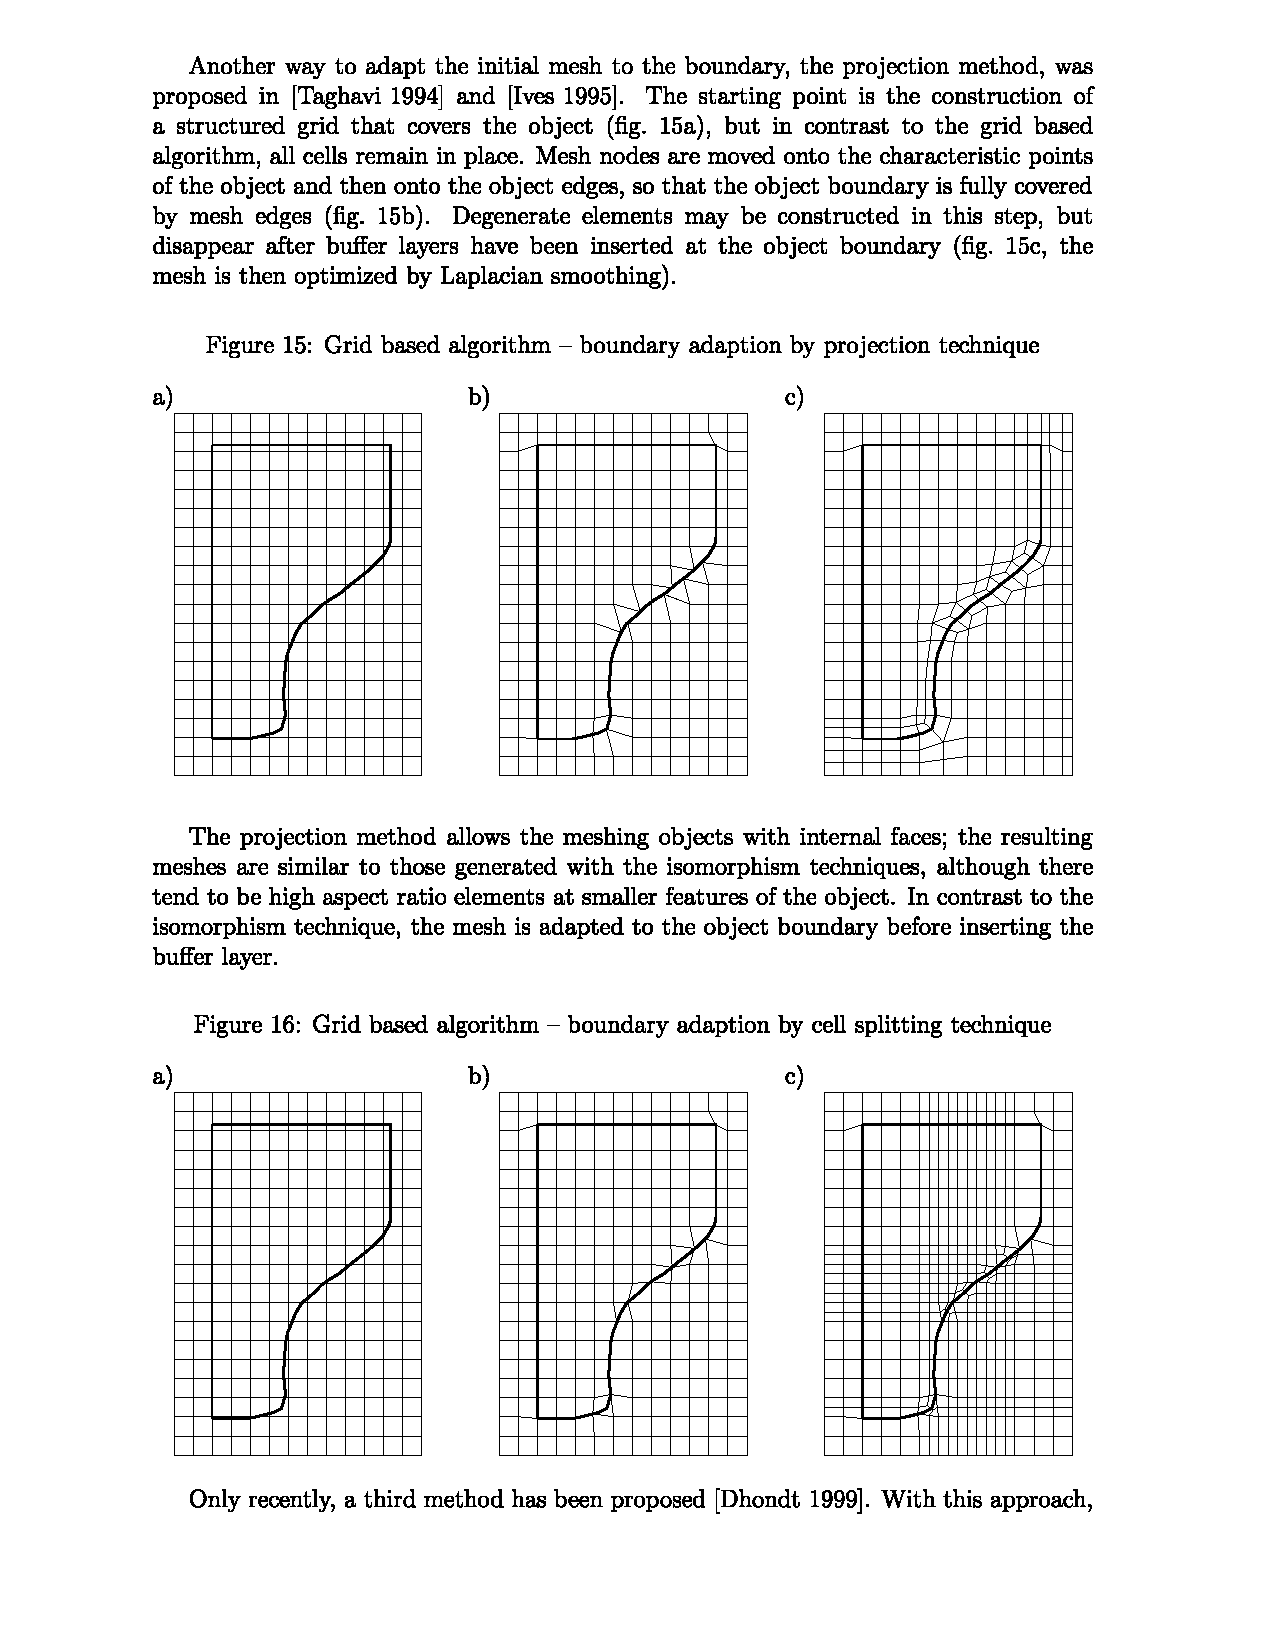
\includegraphics[width=0.325\linewidth]{grid}
}
\subfloat[初始]{
\includegraphics[width=0.325\linewidth]{init}
}
\subfloat[结果]{
\includegraphics[width=0.325\linewidth]{final}
}
}
\vspace{-2mm}
\caption{可视化例子1中的各向异性。 (a) 在定义域中的目标各向异性,使用椭圆来表示。 (b) 初始网格上的$H_\tau$。 (c) 收敛后的$H_\tau$。 结果上的各向异性和目标很接近。}
\label{fig:2daniso}
\vspace{-3mm}
\end{figure}

\begin{figure}[!h]
\centerline
{
\subfloat[BAMG]{
\includegraphics[width=0.37\columnwidth]{fem++_tanh}
}
\subfloat[LCT]{
\includegraphics[width=0.37\columnwidth]{ours_tanh}
}
}
%\vspace{-2mm}
\centerline
{
\subfloat[BAMG]{
\includegraphics[width=0.37\columnwidth]{fem++_cos_x2_y2}
}
\subfloat[LCT]{
\includegraphics[width=0.37\columnwidth]{ours_cos_x2_y2}
}
}
%\vspace{-2mm}
\caption{例子2 -- 与BAMG进行比较。 黎曼度量诱导于非凸解析函数$u(x,y) = \tanh( 10(\sin(5y) -2x)) + x^2 y + y^3$ (上面一行) 和$u(x,y) = e^{3\cos \frac{x^2+y^2}{5}}$ (下面一行)的Hessian矩阵,输入定义域是$[-5.5,5.5]^2$,各向异性比例的范围分别是$[1.9,394.4]$和 $[5.4,597.8]$。 网格三角形的颜色是由面积质量$\qarea$决定的。
}\label{fig:tanh}
\vspace{-3mm}
\end{figure}

我们同时和Zhong等的基于粒子的方法~\cite{Zhong2013}进行比较。对于核函数的宽度值,我们使用了他们推荐值$\sigma$,并且为了实验,选择了两个不同的粒子搜索范围$5\sigma$和$20\sigma$。基于粒子的方法的平均三角形质量比ODT或者LCT差,并且最差的三角形质量($\qtrimin$)远远低于ODT或者LCT。图~\ref{fig:exp}(d)(e)中的颜色也展示了比较差的面积质量。基于粒子的能量只惩罚了粒子之间的黎曼距离的不规则性,但是忽略了三角形之间的关系。

最后, 我们还和Chen的基于ODT的局部区域方法(local patch)~\cite{Chen2004a}进行比较。 它首先在每个顶点$\mp$上,使用平均黎曼度量$\overline{\mathcal{M}}_\mp$构造了一个凸二次函数$u(\mx) = \mx^T \, \overline{\mathcal{M}}_{\mp} \, \mx$。$\overline{\mathcal{M}}_\mp$是在它的一领域中计算的。然后它通过优化局部ODT能量$\int_{\Omega_{\mp}} |u(\mx)-\hat{u}(\mx)|\, \mathrm{d} \mx$,来一个一个的更新每个顶点$\mp$。 如果这个方法使用了局部二次函数,所以与我们的算法相比,会出现相似的结果。但是它没有考虑顶点更新而给其他顶点带来的影响。这个算法有可能不收敛或者收敛到一个不是最优的各向异性网格。图~\ref{fig:exp}(f)展示了~\cite{Chen2004a}的结果,它没有很好的符合指定的各向异性。相比于其他的方法,面积质量,ODT能量很差。 我们注意到将一个顶点周围的所有的局部ODT能量同时优化,~\cite{Chen2004a}结果可以提高。这其实是我们算法的一个变种,二次凸函数是定义在顶点上的,而不是定义在每个三角形上的。
图~\ref{fig:2daniso} 可视化了定义在输入网格和结果上的各向异性。

\textbf{例子2}\quad
图~\ref{fig:tanh}将我们的算法和BAMG进行比较。 BAMG是一个流行的程序,用来生成二维各向异性网格。我们选择了一个方形的区域作为定义域,并且测试了两个从非凸函数诱导的黎曼度量场。BAMG产生了质量比较低的结果,特别是在各向异性变化比较剧烈的区域。为了保证顶点的数目一致和比较的公平,我们将BAMG的输出作为我们的输入,然后使用LCT去优化,从而获得质量提高的结果(见表~\ref{tab:2d}中的质量统计值)。因此我们的算法能够很好的适应变化剧烈的黎曼度量场。

\begin{figure}[t]
\raggedleft
{
\subfloat[各向异性]{
\begin{overpic}[width=0.22\columnwidth]{strech20000}
\put(30,90){$\lambda(\mx)$}
\end{overpic}
}
\subfloat[particle]{
\begin{overpic}[width=0.26\columnwidth]{particle20000}
 \setlength{\fboxrule}{0.5pt}
 \setlength{\fboxsep}{0cm}
\put(12,50){\fbox{\includegraphics[width=0.1\columnwidth]{pzoom}}}
%\put(8,40){\small \contour{white}{zoomed-in view}}
\end{overpic}
\begin{overpic}[width=0.26\columnwidth]{particles}
 \setlength{\fboxrule}{0.5pt}
 \setlength{\fboxsep}{0cm}
\put(45,50){\fbox{\includegraphics[width=0.12\columnwidth]{pzoommesh}}}
%\put(8,40){\small \contour{white}{zoomed-in view}}
\end{overpic}
\begin{overpic}[width=0.22\columnwidth]{hist20000p}
\put(55,90){ $\qangall$}
\put(60,34){ $\qtri$}
\end{overpic}
}
}
\raggedleft
{
\subfloat[LCT]{
\begin{overpic}[width=0.26\columnwidth]{lcvt20000}
 \setlength{\fboxrule}{0.5pt}
 \setlength{\fboxsep}{0cm}
\put(12,50){\fbox{\includegraphics[width=0.1\columnwidth]{ourzoom}}}
%\put(8,40){\small \contour{white}{zoomed-in view}}
\end{overpic}
\begin{overpic}[width=0.26\columnwidth]{lcvt}
 \setlength{\fboxrule}{0.5pt}
 \setlength{\fboxsep}{0cm}
\put(45,50){\fbox{\includegraphics[width=0.12\columnwidth]{ourzoommesh}}}
%\put(8,40){\small \contour{white}{zoomed-in view}}
\end{overpic}
\begin{overpic}[width=0.22\columnwidth]{hist20000lcot}
\put(55,90){ $\qangall$}
\put(60,34){ $\qtri$}
\end{overpic}
}
}
%\centerline{\small
%(a) Stretch(x)  (b) Our point result  (c) Our mesh result  (d) Zhong \etal's point result (e) Zhong \etal's mesh result
%}
\caption{例子3 -- 和Zhong的基于粒子的方法~\cite{Zhong2013}法进行比较。 粒子法(b)和我们的方法(c) 使用了一个圆盘对称的各向异性比例$\lambda(\mx)$,显示在(a)中。 从左到右,我们比较了点的分布,面积质量$\qarea$,和角度质量与三角形质量的直方图。从点的分布与网格的局部放大的图,可以看出我们的结果变换的更加平缓,和指定的各向异性更加贴合,并且生成了更加规则的网格。我们的算法可以获得更好的角度质量$\qangall$(我们的结果更加聚在最优值60$^\circ$附近)和三角形质量$\qtri$(我们的结果更加聚在最优值1),可以直接从右端的直方图中体现。
}\label{fig:particlecompare2d}
\vspace{-3mm}
\end{figure}

\textbf{例子3}\quad
图~\ref{fig:particlecompare2d} 展示了另一个和Zhong的基于粒子的方法~\cite{Zhong2013}比较的结果。在定义域$[-100,100]^2$上,各向异性是通过一个圆盘黎曼度量场决定的:
$$\mathcal{M}(\mx) = Q(\mx) \, \diag(\lambda^2(\|\mx\|), 1) \, Q^T(\mx),$$
其中$\lambda \in [1,10]$,如图~\ref{fig:particlecompare2d}(a)所示。
20000个顶点在这个定义域内被采样,这个数目是来自~\cite{Zhong2013}的结果。 我们的算法使用了31秒,然而~\cite{Zhong2013}使用了20分钟左右。从图~\ref{fig:particlecompare2d}中的很容易看出,LCT获得了较好的结果,更好的顶点分布,更好的网格质量(同时见表~\ref{tab:2d})。

\textbf{例子4}\quad
LCT能量优化可以被认为是一种网格平滑,所以很自然的和其他的光滑函数优化进行比较。我们选择了三种流行的能量。
\begin{itemize}
\item 1.将所有的各向异性的边长的平方和累加:$E_1 \triangleq \sum |e_\Minv|^2$;
\item 2.将每个三角形的各向异性的边长的平方和用面积归一化后累加: $E_2 \triangleq \sum_\tau \frac{\sum_{\me \in \tau} |e_\Minv|^2}{|\tau|}$;
\item 3.将每个三角形的各向异性的边长的平方累乘用面积归一化后累加:$E_3 \triangleq \sum_\tau \frac{\prod_{\me \in \tau} |e_\Minv|}{|\tau|}$。
\end{itemize}
这三种能量都来自~\cite{Shewchuk2002}。
在顶点的更新和三角形网格边翻转中,将$E_1$, $E_2$ or $E_3$代替LCT能量。初始网格由我们的边长规则化策略产生。图~\ref{fig:energy}和表~\ref{tab:2d}显示了,相比于LCT能量,优化$E_1$或者$E_2$可以提高更小的网格质量,然而优化$E_3$反而降低了初始网格的质量。

\begin{figure}[t]
\centerline
{
\subfloat[initial mesh]{
\includegraphics[width=0.33\columnwidth]{input_mesh}
}
\hfill
\subfloat[optimizing $E_1$]{
\includegraphics[width=0.33\columnwidth]{energy_no_area}
}
\hfill
\subfloat[optimizing $E_2$]{
\includegraphics[width=0.33\columnwidth]{energy_divide_area}
}
}
%\vspace{-2mm}
\centerline{
\subfloat[optimizing $E_3$]{
\includegraphics[width=0.33\columnwidth]{energy_edgemul}
}
\qquad
\subfloat[optimizing LCT]{
\includegraphics[width=0.33\columnwidth]{energy_lcvt}
}
}
\vspace{-2mm}
\caption{例子四 -- 和其他的光滑函数比较。 黎曼度量是诱导于$u(x,y)=e^{\sin x + \cos y}$,各向异性比例范围是$[1,429]$。 网格最后使用面积质量$\qarea$着色。
}
\label{fig:energy}
\vspace{-3mm}
\end{figure}

\begin{table}[!h]
\caption{例子2,3,4的质量统计。}
\centering \scalebox{0.9}{
\begin{tabular}{lrcccc}%|l}
  \toprule
  % after \\: \hline or \cline{col1-col2} \cline{col3-col4} ...
   &\#vert & $\lambda$&$\qtrimin/\qtriavg/\qtridev$ & $\qangmin/\qangavg/\qangdev$ & $r_6$ \\% & $r_\angle$   \\
   \midrule
  Fig.~\ref{fig:tanh}a (BAMG)  & 1289 &[1.9,394.4]& 0.22/0.83/0.13 & $10.3^\circ/46.4^\circ/8.9^\circ$ & 0.60 \\%& 0.31 \\
  Fig.~\ref{fig:tanh}b (LCT)  & 1289 &[1.9,394.4]& \textbf{0.42}/\textbf{0.89}/\textbf{0.08} & $\textbf{22.8}^\circ/\textbf{50.4}^\circ/\textbf{5.8}^\circ$ & \textbf{0.69} \\%& \textbf{0.32} \\
   \midrule
  Fig.~\ref{fig:tanh}c (BAMG)  & 6251 &[5.4,597.8]& 0.07/0.87/0.08  & $3.9^\circ/49.6^\circ/6.0^\circ$ & 0.60 \\%& 0.19 \\
  Fig.~\ref{fig:tanh}d (LCT)  & 6251 &[5.4,597.8] & \textbf{0.45}/\textbf{0.90}/\textbf{0.07} & $\textbf{21.1}^\circ/\textbf{51.3}^\circ/\textbf{5.2}^\circ$ & \textbf{0.70} \\%& 0.19 \\
   \midrule
  Fig.~\ref{fig:particlecompare2d} (particle) & 20000 &[1,10] & 0.09/0.90/0.08 & $6.1^\circ/52.5^\circ/5.0^\circ$ & 0.78 \\%&0.19\\
  Fig.~\ref{fig:particlecompare2d} (LCT) & 20000 &[1,10]& \textbf{0.57}/\textbf{0.94}/\textbf{0.04} & $\textbf{31.0}^\circ/\textbf{54.5}^\circ/\textbf{3.3}^\circ$ & \textbf{0.90} \\%& \textbf{0.38} \\
   \midrule
  Fig.~\ref{fig:energy}a (init) & 2316 &[1,429] & 0.32/0.80/0.11 & $14.5^\circ/44.4^\circ/7.3^\circ$ & \textbf{0.67} \\%& 0.67 \\
  Fig.~\ref{fig:energy}b ($E_1$) & 2316 &[1,429]& 0.38/0.86/0.09 & $23.4^\circ/48.5^\circ/6.3^\circ$ & 0.40\\%& 0.77\\
  Fig.~\ref{fig:energy}c ($E_2$) & 2316&[1,429] & 0.42/0.87/0.08 & $25.4^\circ/49.4^\circ/5.6^\circ$ & 0.41 \\%& 0.80 \\
  Fig.~\ref{fig:energy}d ($E_3$) & 2316&[1,429] & 0.15/0.80/0.13 & $6.4^\circ/44.4^\circ/8.7^\circ$ & 0.38 \\
  Fig.~\ref{fig:energy}e (LCT) & 2316 &[1,429]& \textbf{0.60}/\textbf{0.91}/\textbf{0.06} & $\textbf{32.5}^\circ/\textbf{52.6}^\circ/\textbf{4.6}^\circ$ & 0.64 \\%& \textbf{0.84} \\
   \bottomrule
\end{tabular}
}
\label{tab:2d}\vspace{-4mm}
\end{table}

\subsection{三维各向异性曲面网格生成}
\begin{figure}[t]
\centerline
{
\includegraphics[width=1\columnwidth]{surf}
}
\vspace{-5pt}
\caption{使用我们的算法生成的各向异性三维曲面模型(Beetle, Rockarm 和 Hand)。}
\label{fig:nofeature}\vspace{-5mm}
\end{figure}

\begin{figure}[t]
\centerline
{
\begin{overpic}[width=1\columnwidth]{feature3}
%\put(22,6){\small angle}
%\put(56,6){\small angle}
%\put(90,6){\small angle}
\end{overpic}
}
\vspace{-5pt}
\caption{使用我们的算法应用到带有尖锐特征的各向异性曲面网格生成中(Block, Impeller 和 Fandisk)。  }\label{fig:feature}\vspace{-5mm}
\end{figure}

图~\ref{fig:nofeature}展示一些曲面的结果(Beetle, Rockarm, Hand 模型),各向异性是通过曲面的曲率决定的。 对于这三个模型,我们的方法分别使用64, 17 和77秒生成高质量的结果(见表~\ref{table:stat})。我们将LCT应用到有尖锐特征的曲面上,如图~\ref{fig:feature}所示。

\begin{figure}[t]
\centerline
{
\begin{overpic}[width=1\columnwidth]{cyclide}
\put(25,7){ $\qangall$}
\put(59,7){ $\qangall$}
\put(93,7){ $\qangall$}
\end{overpic}
}
\centerline
{
\textbf{(a)} ACVT \hspace{0.15\linewidth} \textbf{(b)} particle \hspace{0.15\linewidth} \textbf{(c)} LCT
}
\caption{在Cyclide模型上,和ACVT~\cite{Valette2008}与基于粒子的方法~\protect\cite{Zhong2013}进行比较。从放大的局部图和直方图来看,我们的结果要远好于它们。
%\jms{Hard to see whether the angular histogram is an better for us than Zhong.}
%\jms{Center labels!}
}\label{fig:cyclide}
\vspace{-3mm}
\end{figure}

图~\ref{fig:cyclide} 将我们的算法和ACVT~\cite{Valette2008}, 基于粒子的方法~\cite{Zhong2013}在Cyclide模型上进行比较。ACVT生成了很差的结果:$16.8\%$ 的三角形拥有小于$30^\circ$的角。基于粒子的算法稍微好点,但是相比于我们,质量还是差了很多。比如我们的度为6的顶点比例,基于粒子的算法和ACVT分别为: 0.87,0.78,0.51。同时我们能获得更好的三角形和角度质量,见表~\ref{table:stat}中更多的数据。

\begin{figure}[!h]
\centerline
{
\begin{overpic}[width=1\columnwidth]{Fertilitynew}
\put(20,51){  ACVT}
\put(65,51){  ADR}
\put(20,-3){  particle}
\put(65,-3){  LCT}
\end{overpic}
}
\vspace{3mm}
\caption{和ACVT~\protect\cite{Valette2008},基于粒子的方法~\protect\cite{Zhong2013}, 与ADR~\protect\cite{Boissonnat2013} 在模型Fertility上比较。放大的局部图很好的展示结果的差别,说明我们的方法能获得更好质量的结果。 }
\label{fig:fertility}
\vspace{-3mm}
\end{figure}

\begin{table}[t]
\caption{生成各向异性曲面网格的质量和时间统计。我们列出了参考网格的顶点数目(“ref \#vert”),初始网格的顶点数目(“init \#vert”),输出网格的顶点数目(“\#vert”)。$\lambda$是各向异性比例的范围。$\%_{<30^{\circ}}$是三角形的最小角小于$30^\circ$的比例。$\dis_{H}$是参考网格与输出网格之间的Hausdorff距离与参考网格包围盒的对角线长度之间的比例。对于ACVT方法,参考网格被细分用来提供更好的近似精度。基于粒子的方法和ADR的数据是来自于\protect\cite{Zhong2013}。
}
\centering \scalebox{0.6}{
\begin{tabular}{lrrrcccrccr}%|r}
\toprule
模型               & ref \#vert & init \#vert & \#vert & $\lambda$ & $\qtrimin/\qtriavg/\qtridev$ & $\qangmin/\qangavg/\qangdev$ & $\%_{<30^{\circ}}$ & $\dis_{H}$ & $r_6$ %& $r_\angle$
& time (s) \\
\midrule
Cyclide (particle) & -     & 8000   & 8000   & $[2, 29]$  & 0.09/0.87/-      & $5.03^\circ/49.7^\circ/-^\circ$   & \textbf{0.04}\%   & 4.4e-4        & 0.78 %& 0.06
& 155.8             \\
Cyclide (ACVT) & 414720    & 8000    & 8009    & $[2, 29]$ & 0.002/0.75/0.17  & $0.07^\circ/40.8^\circ/10.8^\circ$   & 16.8\%            & 3.6e-3         & 0.51 %& 0.26
& 177.0             \\
%Cyclide (ACVT) & 414720    & 8000    & 8000     & ?      & ?      & $?^\circ$   & $?^\circ$   & ?\%            & $?\times10^{-2}$         & 0.46 & ?      & 154.3             \\
Cyclide (LCT)     & 25920     & 8000   & 8000    & $[2, 29]$  & \textbf{0.60}/\textbf{0.92}/\textbf{0.05}
    & $\textbf{26.9}^\circ/\textbf{53.1}^\circ/\textbf{4.2}^\circ$   & \textbf{0.03}\%            & \textbf{3.4e-4}       & \textbf{0.87} %& \textbf{0.35}
         & \textbf{17.5}         \\
\midrule
Fertility (ACVT) & 223626     & 12480   & 12480   & $[1, 14]$   & 0.00/0.67/0.19      & $0.12^\circ/35.6^\circ/11.7^\circ$   & 32.67\%            & \textbf{1.1e-3}        & 0.39 %& 0.57
      & 37.5             \\
%Fertility (ACVT) & 223626     & 12480   & 12480     & 0.002      & 0.67      & $0.12^\circ$   & $35.6^\circ$   & 32.67\%            & $1.1\times10^{-3}$         & 0.26 & 0.57        & 58.8            \\
Fertility (ADR) & -     & 12480   & 12480   & $[1, 14]$   & 0.002/0.56/-      & $0.06^\circ/29.9^\circ/-^\circ$   & 41.79\%            & 5.8e-3       & 0.46 %& 0.38
    & - \\
    %& {\raise.17ex\hbox{$\scriptstyle\sim$}}400            \\
Fertility (particle) &-   & 12480     & 12301  & $[1, 14]$    & 0.02/0.70/-      & $0.86^\circ/37.6^\circ/-^\circ$   & 26.99\%            & 2.3e-3          & 0.49 %&  0.28
 & \textbf{10.0}           \\
Fertility (LCT)     & 13971   & 12480     & 12480  & $[1, 14]$   & \textbf{0.54}/\textbf{0.89}/\textbf{0.07}
& $\textbf{24.9}^\circ/\textbf{50.8}^\circ/\textbf{5.1}^\circ$   & \textbf{0.04}\%           & \textbf{1.1e-3}      & \textbf{0.68} %&\textbf{0.65}
& 66.8         \\
\midrule

Rockarm               & 9413  & 1272       & 5550  & $[1, 18]$    & 0.34/0.86/0.08      & $20.4^\circ/48.9^\circ/6.1^\circ$   & 0.46\%             & 1.8e-3       & 0.60 %& 0.63
   & 17.6           \\
Fandisk             & 6475    & 1927     & 7950   & $[1, 15]$   & 0.14/0.87/0.08      & $8.4^\circ/48.9^\circ/5.8^\circ$   & 0.18\%             & 9.5e-4       & 0.60 %&  0.51
   & 19.6           \\
Beetle            & 17908      & 17908      & 9817   & $[1, 15]$   & 0.27/0.87/0.08      & $13.2^\circ/48.9^\circ/6.0^\circ$   & 0.66\%     & 9.2e-4    & 0.52 %& 0.53
&   64.3  \\
Block               & 8052    & 3307     & 11667  & $[1, 15]$    & 0.51/0.88/0.07      & $27.2^\circ/50.1^\circ/5.4^\circ$   & 0.03\%             & 1.1e-3        & 0.63 %& 0.66
   & 38.7           \\
Impeller            & 10000  & 10000      & 11737   & $[1, 16]$   & 0.39/0.87/0.08      & $22.1^\circ/49.6^\circ/5.8^\circ$   & 0.17\%             & 6.5e-4      & 0.60 %& 0.40
    & 110.5          \\
Botijo              & 14989   & 700     & 13890  & $[1, 16]$    & 0.52/0.89/0.07      & $23.1^\circ/50.9^\circ/5.0^\circ$   & 0.04\%             & 1.6e-3      & 0.66 %& 0.75
    & 39.1         \\
Hand                & 30000  & 2576     & 21226  & $[1, 14]$   & 0.46/0.90/0.06      & $20.6^\circ/51.4^\circ/4.8^\circ$   & 0.04\%             & 1.1e-3    & 0.67% & 0.60
     & 77.1          \\
%Buddha        & 115474    & 5000   & 63284  & $[1, 34]$ & 0.41/0.88/0.07  & $17.4^\circ/49.9^\circ/5.4^\circ$   & 0.03\%           & 6.7e-4      & 0.64 %& 0.56 & 178.5         \\
%Lucy                & 262787    & 74119  & 255097   & $[1, 19]$   & 0.26/0.90/0.06      & $15.4^\circ/51.4^\circ/5.0^\circ$   & 0.04\%             & 3.9e-4    & 0.70% & 0.60  & 2766.0          \\
\bottomrule
\end{tabular}}
\label{table:stat}\vspace{-5mm}
\end{table}

\begin{figure}[b]
\centerline
{
\begin{overpic}[width=0.95\columnwidth]{planar}
\put(93,74){  $\qangall$}
\put(93,55){  $\qre$}
\put(33,40){MMG3D}
\put(93,30){  $\qangall$}
\put(93,12){  $\qre$}
\put(35,0){LCT}
\end{overpic}
}
\vspace{2mm}
\vspace{-8pt}
\caption{简单的各向异性四面体网格生成例子。黎曼度量场是$\mathcal{M}(\mx)=\Lambda^2(\mx)$,其中$\Lambda(\mx) = \diag\left((0.0025+0.2(1-e^{-|x-0.6|}))^{-1}, 5, 5 \right)$。
中间的图像是四面体网格的切面图,展示了内部四面体的情况。右边的图像是所有的二面角$\qangall$和半径-边长比例$\qre$的直方图。我们的算法提供了离最优值(70.5$^\circ$ 对于 $\qangall$, 0.61 对于 $\qre$)更紧的分布。
}\label{fig:planartet}
\vspace{-3mm}
\end{figure}

图~\ref{fig:fertility} 将我们的算法和ACVT~\cite{Valette2008},基于粒子的算法和ADR~\cite{Boissonnat2013}在Fertility模型上进行比较。目标的黎曼度量是由曲面的曲率决定的。基于粒子的算法跑了100次迭代,并且使用并行进行加速。目标输出的顶点数目是和ADR的输出一致的。我们的算法可以获得更好的网格正则度,对原始的网格的近似更加合理(见表~\ref{table:stat}中的Hausdorff距离)。对于角度和三角形质量,LCT获得了更好的质量,更好的贴合了到处的各向异性。

\subsection{各向异性四面体网格生成}

\begin{figure}[t]
\centerline
{
\begin{overpic}[width=0.95\columnwidth]{cylinder}
\put(93,74){  $\qangall$}
\put(93,55){  $\qre$}
\put(33,40){MMG3D}
\put(93,34){  $\qangall$}
\put(93,17){  $\qre$}
\put(35,0){LCT}
\end{overpic}
}
\caption{另外一个简单的体网格生例子,各向异性是类似圆柱变化的。黎曼度量是$\mathcal{M}(\mx)=\mQ^T(\mx) \, \Lambda^2(\mx) \, \mQ(\mx)$,其中$\Lambda(\mx) = \diag\left(2(0.1+2(1-e^{-0.01|x^2+y^2-49|}))^{-1}, 1, 1\right)$,$\mQ$的三列是 $(x/\sqrt{x^2+y^2}, y/\sqrt{x^2+y^2}, 0)^T$,
$(-y/\sqrt{x^2+y^2}, x/\sqrt{x^2+y^2}, 0)^T$和$(0,0,1)^T$。
}\label{fig:cylindertet} \vspace{-3mm}
\end{figure}

\begin{figure}[t]
\centerline
{
\begin{overpic}[width=0.95\columnwidth]{sine}
\put(93,65){  $\qangall$}
\put(93,48){  $\qre$}
\put(31,37){MMG3D}
\put(93,29){  $\qangall$}
\put(93,12){  $\qre$}
\put(33,0){LCT}
\end{overpic}
}
\caption{一个球内的正弦各向异性。黎曼度量是$\mathcal{M}(\mx)=\mQ^T(\mx) \, \Lambda \, \mQ(\mx)$,其中$\Lambda = \diag(1000,10,10)$, $\mQ$的三列是$(2\cos(6x),1,0)^T$和两个相互正交的向量。
}\label{fig:sinetet} \vspace{-3mm}
\end{figure}

\begin{figure}[t]
\centerline
{
\begin{overpic}[width=0.95\columnwidth]{bump}
\put(93,33){  $\qangall$}
\put(93,12){  $\qre$}
\end{overpic}
}
\caption{在一个复杂的bumpy形状中的圆柱各向异性。目标各向异性使用和图~\ref{fig:cylindertet}一样的$\mQ$,但是
$\Lambda_1(\mx) =1.2/(0.5 + 1 - e^{-0.05(x^2+y^2 - 2.56)}),\:
\Lambda_2(\mx)=\Lambda_3(\mx)=\Lambda_1(\mx)\,(1+5\sqrt{x^2+y^2})$。
}\label{fig:bump} \vspace{-3mm}
\end{figure}

图~\ref{fig:planartet}和~\ref{fig:cylindertet}将我们的算法和MMG3D相比。定义域是一个立方体$[0.1,1.1]^3$ (图~\ref{fig:planartet})或者$[1,11]^3$(图~\ref{fig:cylindertet})。两个结果的网格质量是类似的(见表~\ref{table:tetstat})。相比于MMG3D,从直方图与表中的统计信息可以看出我们的算法能够获得更好的角度和半径-边长比($\qre$)质量。并且网格质量的标准差也比MMG3D好。注意和MMG3D相比,我们的四面体网格拥有更加稀疏的四面体数量(1870顶点 vs. 2365 顶点在图~\ref{fig:planartet}中, 6338顶点 vs. 8217顶点在图~\ref{fig:cylindertet}中)。图~\ref{fig:sinetet}展示了另一个和MMG3D比较的例子,定义域是一个单位球,两个算法使用相同的表面作为输入。我们的算法可以生成更少的sliver四面体,更好的角度和半径-边长比质量。我们的算法比MMG3D慢,因为比较低效率的翻边实现,和串行的顶点更新。

我们在MMG3D的结果上,跑了100次迭代的LCT优化和一个最后的sliver四面体去除过程。结果同样被列在表~\ref{table:tetstat}中,命名为“MMG3D-LCT”。LCT能提高网格的角度和半径-边长比质量。

图~\ref{fig:bump}展示了一个更多体网格生成的结果。三维定义域是一个bumpy形状,各向异性是由一个解析函数决定的。 目标各向异性为
\begin{equation}
\Lambda(\mx) = \diag\left((0.025+(1-e^{-0.01|\|\mx\|^2-49|}))^{-1},1,1\right),
\end{equation}
$\mQ$的三列是$\mx/\|\mx\|$和两个相互正交的向量。 定义域是一个立方体$[1,11]^3$。

\begin{table}[t]
\caption{四面体各向异性网格生成的数据和时间统计。\#sliver$_b$和\#sliver$_a$是实施sliver四面体去除策略前与后的数量。}
\centering \scalebox{0.6}{
\begin{tabular}{lrrrcccrrr}
\toprule
Model & init \#vert & \#vert & \#tet & $\lambda$ & $\qangmin/\qangavg/\qangdev$ & $\qre_{max}/\qre_{avg}/\qre_{dev}$   & \#sliver$_b$ & \#sliver$_a$ & time (s) \\
\midrule
Fig.~\ref{fig:planartet} (LCT)    & 948   & \textbf{1870}  & \textbf{8144}  & $[1, 80]$  &$\textbf{24.7}^\circ/\textbf{51.7}^\circ/7.5^\circ$ &1.46/\textbf{0.76}/0.07  & 71  &  0   &   8.3  \\
Fig.~\ref{fig:planartet} (MMG3D)  & -     & 2365  & 10860 & $[1, 80]$  &$22.0^\circ/48.1^\circ/7.7^\circ$ &1.37/0.83/0.09  & -    &  0   &   \textbf{4.9} \\
MMG3D-LCT  & -     & 2365  & 10913 & $[1, 80]$  &$22.6^\circ/51.5^\circ/7.8^\circ$ &\textbf{1.36}/0.77/0.07  & 23    &  0   &   5.1 \\
\midrule
Fig.~\ref{fig:cylindertet} (LCT)  & 2226  & \textbf{6338}  & \textbf{31840} & $[1, 20]$  &$17.7^\circ/50.6^\circ/8.5^\circ$ &\textbf{1.54}/0.78/0.08  & 517  &  0   &   72.6 \\
Fig.~\ref{fig:cylindertet} (MMG3D)& -     & 8217  & 42067 & $[1, 20]$  &$16.2^\circ/46.8^\circ/8.2^\circ$ &2.59/0.86/0.13  & -    &  0   &   \textbf{15.4} \\
MMG3D-LCT  & -     & 8217  & 42435 & $[1, 20]$  &$\textbf{18.1}^\circ/\textbf{50.9}^\circ/8.6^\circ$ &1.71/\textbf{0.77}/0.09  & 530    &  0   &   31.2 \\
\midrule
Fig.~\ref{fig:sinetet} (LCT)      & 1966  & \textbf{4739}  & \textbf{22427}& $[1, 10]$  &$9.1^\circ/44.7^\circ/10.7^\circ$ &5.56/0.89/0.18   & 1715 &  72  &   103.8 \\
Fig.~\ref{fig:sinetet} (MMG3D)     & -     & 5187  & 25311& $[1, 10]$  &$6.2^\circ/37.1^\circ/10.9^\circ$ &6.27/1.21/0.41   & -    &  264 &   \textbf{6.5}  \\
MMG3D-LCT  & -     & 5187  & 25767 & $[1, 10]$  &$\textbf{9.4}^\circ/\textbf{44.8}^\circ/10.8^\circ$ &\textbf{3.50}/\textbf{0.88}/0.17  & 1932   &  \textbf{65}   &   33.1 \\
\midrule
%Fig.~\ref{fig:teaser}-right       & 2158  & 6554 & 32668 & $[1, 40]$  &$15.3^\circ/48.9^\circ/9.2^\circ$ &2.80/0.83/0.13   & 844   &  0  & 104.6 \\
Fig.~\ref{fig:bump}      & 18183  & 35096  & 153959 & $[1, 13]$  &$15.3^\circ/51.1^\circ/8.3^\circ$ &1.41/0.77/0.07   & 534  &  0   &   339.4 \\
\bottomrule
\end{tabular}}
\label{table:tetstat} \vspace{-3mm}
\end{table}

\section{本章小结}
局部凸函数三角化(LCT)提供了一个新颖的、简单的算法来生成二维平面区域,三维曲面区域和三维体区域上的高质量各向异性网格。我们的算法继承了ODT的优点,并且推广它能适用于一般的黎曼度量场。它提供了高效率和极好的网格质量。当然我们的算法存在一些局限性,供未来的工作来解决。

\paragraph{网格质量的界}
与\cite{Labelle2003,Boissonnat2008a}相比,我们不能对网格质量提供严格保证。一个可能的解决思路是结合\cite{Boissonnat2008a}的各向异性Delaunay细化和我们的LCT优化,来给最坏的网格质量提供界限,并且保持我们算法的平均质量。另外最小化最大误差$E_{LCT,\infty}$也是另外一个思路来控制最差质量。

\paragraph{凸局部函数}
和Chen等的方法~\cite{Chen2007}一样,我们的方法通过公式~\ref{eqn:funcmetric}将一个负定的Hessian矩阵转换成正定。当函数$u$是局部非凸时,我们的方法会降低对原始函数的逼近程度。应该使用一个更一般的,而不是公式~\ref{eqn:u_tau}中的$H$。这样一个一般的LCT形式能提供更高的逼近程度,但是会使得优化更加复杂。另外一个可能性是将二次凸函数换成一个更一般的凸函数,能够更好地匹配局部黎曼度量,比如Bernstein-B\'{e}zier样条。



